\chapter{Automatizált Internet mérő rendszer}
%(13-15 oldal): 

Jelen fejezet mutatja be az elkészült automatizált mérési rendszert, annak felépítését és működési elvét.

\section{Mérési elrendezés}
%(5 oldal): traceroute, iperf, mérési forgatókönyvek, PlanetLab

A felhőben vagy kliensen futó szoftver óránként felméri a PlanetLab hálózat gépeinek elérhetőségét és a kapott adatokat, statisztikákat eltárolja az adatbázisában. A PlanetLab hálózatában ugyanis elméleti szinten 1200 körüli végpont van, azonban ezeknek nagy százaléka elérhetetlen. A külön lépésben való feltérképezéssel rengeteg sikertelen kapcsolódást kerül el a mérőrendszer. A csatlakozásra képes célgépekre SSH kapcsolaton keresztül felcsatlakozik. Az egyes mérési forgatókönyveknek megfelelően parancssorozatokat futtat, majd azok eredményeit adatbázisban tárolja.
A nyers mérési eredmények, mint például a traceroute kimenet, később további feldolgozási lépéseken mennek keresztül. Végül az egyes kimutatásokhoz további statisztikák készülnek.
Az alábbiakban ezen lépések kerülnek részletesebb bemutatásra.

\subsection{A méréshez használt hálózat}

Az Interneten végzett mérésekhez szükséges a hálózatok különböző pontjain végezni méréseket. Egyes mérésekhez elegendő egy végpontból elvégezni a méréseket, azonban az csak lokális képet ad vissza, így torzítja az egész Internetről alkotott képet. A mérési rendszer üzemeltetéséhez ezért szükséges volt hozzáférést szerezni további a hálózatban résztvevő csomóponthoz. Így minél több résztvevő szolgáltat mérési adatokat, annál egységesebb képet tudunk kapni a kinyert adatokból. Az előző \ref{internet-measurement} szekcióban bemutatott hasonló mérési rendszerek szintén kiterjedt mérési hálózattal rendelkeztek. A PlanetLab hálózata kézenfekvő megoldás az Internetes mérések végzéséhez. Kiterjedésének nagysága biztosítja a mérés reprezentativitását, valamint megbízhatósága garantálja a mérések sikerességét.

A mérési rendszer azért jöhetett létre, mert a Budapesti Műszaki és Gazdaságtudományi Egyetem, ahol a Diplomamunkámat végeztem, résztvevője a PlanetLab szervezetnek. A részvételhez szükséges volt a megfelelő kapcsolattartó személyek kinevezése és a hálózat számára elérhetővé tenni két szerver gépet, amelyek megfelelnek a követelményeknek. A redundancia érdekében kötelező a két független gép. A hardveres paramétereken felül feltétel volt a szervezet által fejlesztett Linux disztribúció telepítése, amely fel van készítve a megfelelő virtualizáció támogatására. A tudományos mérések izolációjához szükséges a virtualizáció, így ha a szervezet egy résztvevője hibás programot futtat, az nem lesz kihatással a többiek által végzett mérésekre. A hozzáférések biztonságát a kötelező publikus-privát kulcsok használatával garantálják. Miután a mérésekhez generált publikus kulcs feltöltésre került a szervezet központi honlapjára, a mérésekhez már fel is lehetett használni.

A hálózatban elérhető gépekkel kapcsolatban fontos szempont továbbá, hogy hiába van elkülönített virtualizált környezet a résztvevők számára, azokon nem lehet tárolni adatokat. Bármikor felszólítás nélkül új virtualizált környezetet osztanak ki a felhasználók számára. Ezzel biztosítják a szerverek elérhetőségét és a folyamatos tisztulását. A Mérési rendszer készítésekor részben ezért volt szükséges az egyes mérési eredmények azonnali tárolása adatbázisban.

\subsection{Csatlakozás a hálózat számítógépeihez}

A mérések elvégzéséhez szükséges volt a PlanetLab hálózatának gépeihez való automatizált csatlakozás és parancs végrehajtás. A hálózatában résztvevő számítógépek listáját egy központi célgép szolgáltatja.

A mérések elvégzéséhez és feldolgozásához egységesen Python programozási nyelven megírt szkriptek lettek használva. A nyelv rugalmassága, támogatottsága és az elérhető könyvtárak bősége tette alkalmassá a gyors fejlesztésre. 
A méréseket végző program a Paramiko\cite{paramiko} könyvtárat használja az ssh kapcsolatok felépítéséhez és menedzseléséhez. A mérési kísérletek sok esetben hiúsultak meg különböző hibák, vagy a célszámítógép elérhetetlensége miatt, ezért ezen esetek kezelése fontos szempont volt a fejlesztés során. A \ref{fig:statistics} ábrákon látható statisztikák az első mérések adataiból készültek. A mérések óránként lettek elvégezve, lefutásonként 1354 csomóponthoz téve csatlakozási kísérletet. A vezérlő számítógép nem állandóan futott, így egy hónapban csak 23 nap készültek mérések, átlagosan 15 alkalommal.


\begin{figure}[h!]
\begin{center}
    \subfigure[Csatlakozási kísérletek eredményessége]{\label{fig:succeed}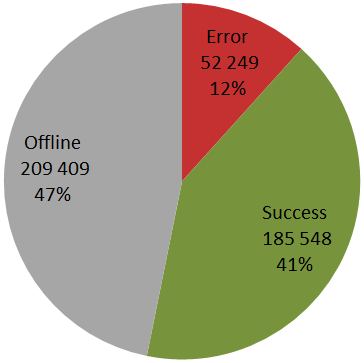
\includegraphics[scale=0.4]{figures/succeed.png}}
    \hspace{10mm}
    \subfigure[Hibák okai]{\label{fig:errors}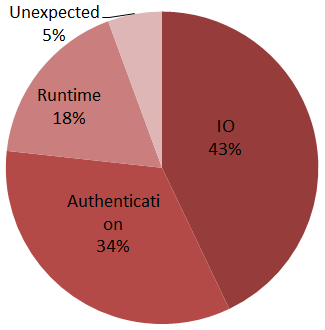
\includegraphics[scale=0.45]{figures/err.png}}
	\caption{Statisztikák\label{fig:statistics}}
\end{center}
\end{figure}

\subsection{Időzített mérési forgatókönyvek}
Az iperf mérések implementálásához új eljárás kidolgozására volt szükség a mérést menedzselő szoftverben. A korábbi traceroute mérések egyetlen parancs távoli futtatásából álltak, amelyek futási eredményét tároltuk el mérési eredményként. Az iperf és más sávszélesség mérő szoftverek működéséhez azonban szükséges mind egy adatcsomagokat küldő és egy adatcsomagokat fogadó példány futtatása a két különböző távoli gépen. Ennek lebonyolításához a mérést lebonyolító programnak több szálon kell futnia, a két távoli kódfuttatást egyszerre kell végeznie. Először az adatcsomagok fogadását (szerver oldal) végző programot kell elindítani, majd csak ezt követően lehet csak a mérést megkezdeni az adatcsomagokat küldő program (kliens oldal) elindításával. A mérést követően a szervert pedig le kell állítani. Ez a szituáció tovább bonyolódik, ha két sávszélesség mérést párhuzamosan szeretnénk végezni. Ez egy fennálló igény, mivel a későbbiekben az MPTCP\footnote{Multipath Transfer Protocol: Több párhuzamos TCP adatfolyamon végez kommunikációt a felsőbb rétegek felé egyetlen TCP kapcsolatot emulálva.} protokoll lehetséges viselkedését is vizsgálni szeretnénk.

Ezeket a lépéseket általánosítva olyan mérési forgatókönyvek létrehozását támogatja már a mérési rendszer, amely bármilyen távoli parancsok időzített futtatását garantálja. Ennek kialakítása a lehető legrugalmasabbra lett tervezve, amelynek működését a függelékben található példakód mutatja be. A kód egyszerűségének ellenére a mérés teljesen menedzselt, bármilyen hiba keletkezése le van kezelve és megfelelően naplózva és a mérési eredményben jelezve van. Garantálva van a helyes időzítés, a párhuzamos futás és a helyes leállás.

%A mérési forgatókönyvek rendkívül hasznosak, segítségükkel új mérések implementálása kényelmes és gyors.


\section{Geolokációs és AS információk}
Az internetes útvonalakat alkotó IP címeknek további fontos tulajdonságai vannak magán a címen kívül. Ezek a mérésekre épülő elemzések, kutatásoknak is fontos, néhol esszenciális alapja. A legegyértelműbb ilyen attribútum, amely az IP címhez köthető az a cím tulajdonosa. A \ref{eroforrasok} szekcióban bemutatott szervezetek publikusan nyilvántartják a szétosztott IP cím erőforrások tulajdonosait. A tulajdonosok minden esetben bejegyzett Autonóm Rendszerek (AS), amelyek azonosító számmal is rendelkeznek. Ezen információkat a mérési rendszer a \href{http://asn.cymru.com/cgi-bin/whois.cgi}{asn.cymru.com} honlap egy publikus szolgáltatásától kéri le. A mérési rendszer kimutatásainak ez az információ fontos része, hisz az Internetet egésze AS hálózatok összességeként értelmezendő. Működésére vonatkozó következtetéseknek fontos eleme kell hogy legyen az Autonóm Rendszerek vizsgálata és egymáshoz viszonyított kapcsolataik. Az egyes Autonóm Rendszerekhez az azonosító számon kívül további információk is elérhetőek, mint például a tulajdonos cég neve, országa.

A mérési rendszernek nem része, azonban a kutatások során használt további publikus szolgáltatások  rendkívül gazdag információkat szolgáltatnak az említett Autonóm Rendszerekről. Az alábbi felsorolás bemutatja ezeket a szolgáltatókat:

\begin{itemize}
\item \textbf{RIPE} Az európai régióért felelős Internet nyilvántartó szervezet honlapja, amely folyamatosan frissen tartott gazdag adatbázisokat nyújt publikusan elérhetően: \linebreak  \href{https://www.ripe.net/manage-ips-and-asns/db}{www.ripe.net/manage-ips-and-asns/db}

\item \textbf{PeeringDB} Egy közösségileg támogatott ingyenes adatbázis Peering információk nyil\-ván\-tar\-tá\-sá\-ra. A Wikipédiához hasonlóan adományokból tartja fenn magát és a regisztrált tagok önkéntes adat hozzájárulásaiból építi fel a folyamatosan növekvő a\-dat\-bá\-zi\-sát. Egy példa a publikusan elérhető adatokról egy ASN-ről:  \linebreak  \href{https://www.peeringdb.com/asn/6939}{www.peeringdb.com/asn/6939}

\item \textbf{Hurricane Electric Internet Services} A legnagyobb IPv6-os hálózattal rendelkező Tier-1-es Internetszolgáltató honlapja, amely rendkívül széleskörűen szolgáltat információkat az Internetes erőforrásokra vonatkozóan. Példa a magyarországi Nemzeti Információs Fejlesztési Iroda AS számáról: \pagebreak
\href{http://bgp.he.net/AS1955}{bgp.he.net/AS1955}
\end{itemize}


Az IP címekkel kapcsolatos további fontos információ azok geológiai elhelyezkedése. Ehhez nincs elérhető hivatalos publikus adatbázis, a korábban említett Regionális Internet Nyilvántartó szervezetek nem kötelezik az általuk kiosztott IP címek további bejegyzését. Ennek ellenére az információ fontossága miatt a világon több szervezet és kutatás foglalkozik mégis az IP címekhez tartozó geolokációs információk összekötésével. Ezek legtöbbje az IP címhez tartozó Autonóm Rendszer bejegyzett elhelyezkedését használja fel, ez azonban sok esetben pontatlan, főleg kiterjedt Autonóm Rendszerek esetében, ahol egyetlen cím van megadva.

\begin{figure}[!ht]
	\centering
	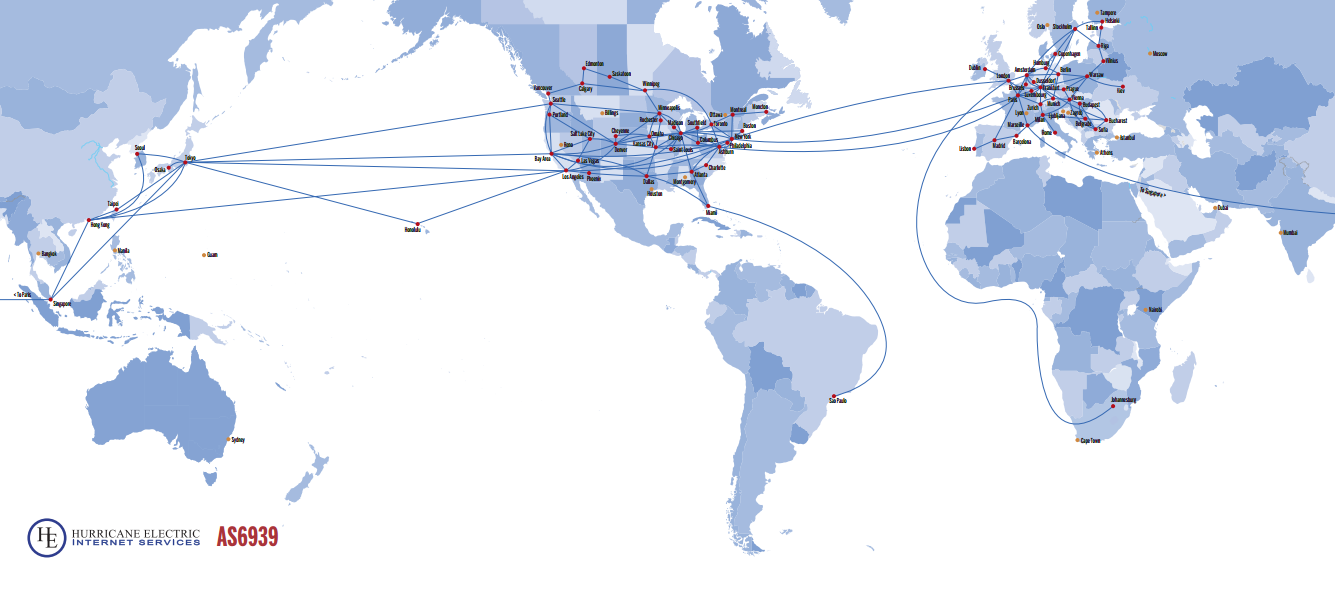
\includegraphics[width=0.8\textwidth, keepaspectratio]{figures/hurricane.png}
	\caption{Egy Tier-1-es Autonóm Rendszer geolokációs kiterjedtsége}
	\label{fig:hurricane}
\end{figure}

A \ref{fig:hurricane} ábrán látható mennyire pontatlan lenne a 6939 számú Autonóm Rendszer alá tartozó IP címeket az Amerikai Fremont városához rendelni Kaliforniában. Ehelyett a fejlettebb IP-geolokációs szolgáltatások Ping késleltetés alapú háromszögeléssel rendelnek szélességi és hosszúsági fokokat az egyes IP címekhez. A legnagyobb ilyen szolgáltató a Maxmind\footnote{\href{https://www.maxmind.com}{www.maxmind.com}} amelynek szolgáltatásait többek között a RIPE is használja.

\begin{figure}[!ht]
	\centering
	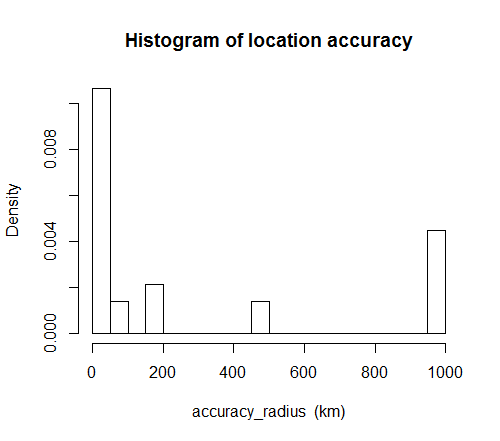
\includegraphics[width=0.7\textwidth, keepaspectratio]{figures/hist-geo.png}
	\caption{A Maxmind GeoLite2 adatbázisának pontosság eloszlása az IP blokkokra vonatkozóan}
	\label{fig:maxmind}
\end{figure}


 Az ilyen típusú adatbázisok az esetek többségében város szintű megbízható pontosságot biztosítanak. A \ref{fig:maxmind} ábrán látható a Maxmind általá ingyenesen elérhető adatbázis pontosságának eloszlása a használatban lévő IP blokkokra vonatkozóan.
A fejlesztett mérési rendszer egy ingyenes szolgáltatást\footnote{\href{https://ipinfo.io}{ipinfo.io}} használt az IP címek helyzetmeghatározásához, mivel a fejlesztés idejében ez tűnt a legmegfelelőbb megoldásnak, az ingyenes Maxmind adatbázis ismerete nélkül.

\pagebreak

Az online szolgáltatásoktól való adatlekérdezések az adatgazdagítás során problémát okoztak a lassú kapcsolatfelépítés és a címek egyenkénti lekérdezése miatt. Emiatt gyorsítótárazási stratégia lett fejlesztve a Python könyvtárakba.
A mérési eredmények és az általuk prezentált információkhoz rendkívül fontos adatforrások voltak az említett információ források felhasználása.
